\documentclass{article}

\usepackage{graphicx}
\usepackage{tikz}
\usepackage{tikzsymbols}
\usetikzlibrary{calc,patterns,shapes.geometric}
\pagestyle{empty}
\usepackage[margin=0pt]{geometry}
\geometry{papersize={14in,12in}}

\def\centerarc[#1](#2)(#3:#4:#5){\draw[#1] ($(#2)+({#5*cos(#3)},{#5*sin(#3)})$) arc (#3:#4:#5);}

\begin{document}
	\begin{figure}
		\centering
		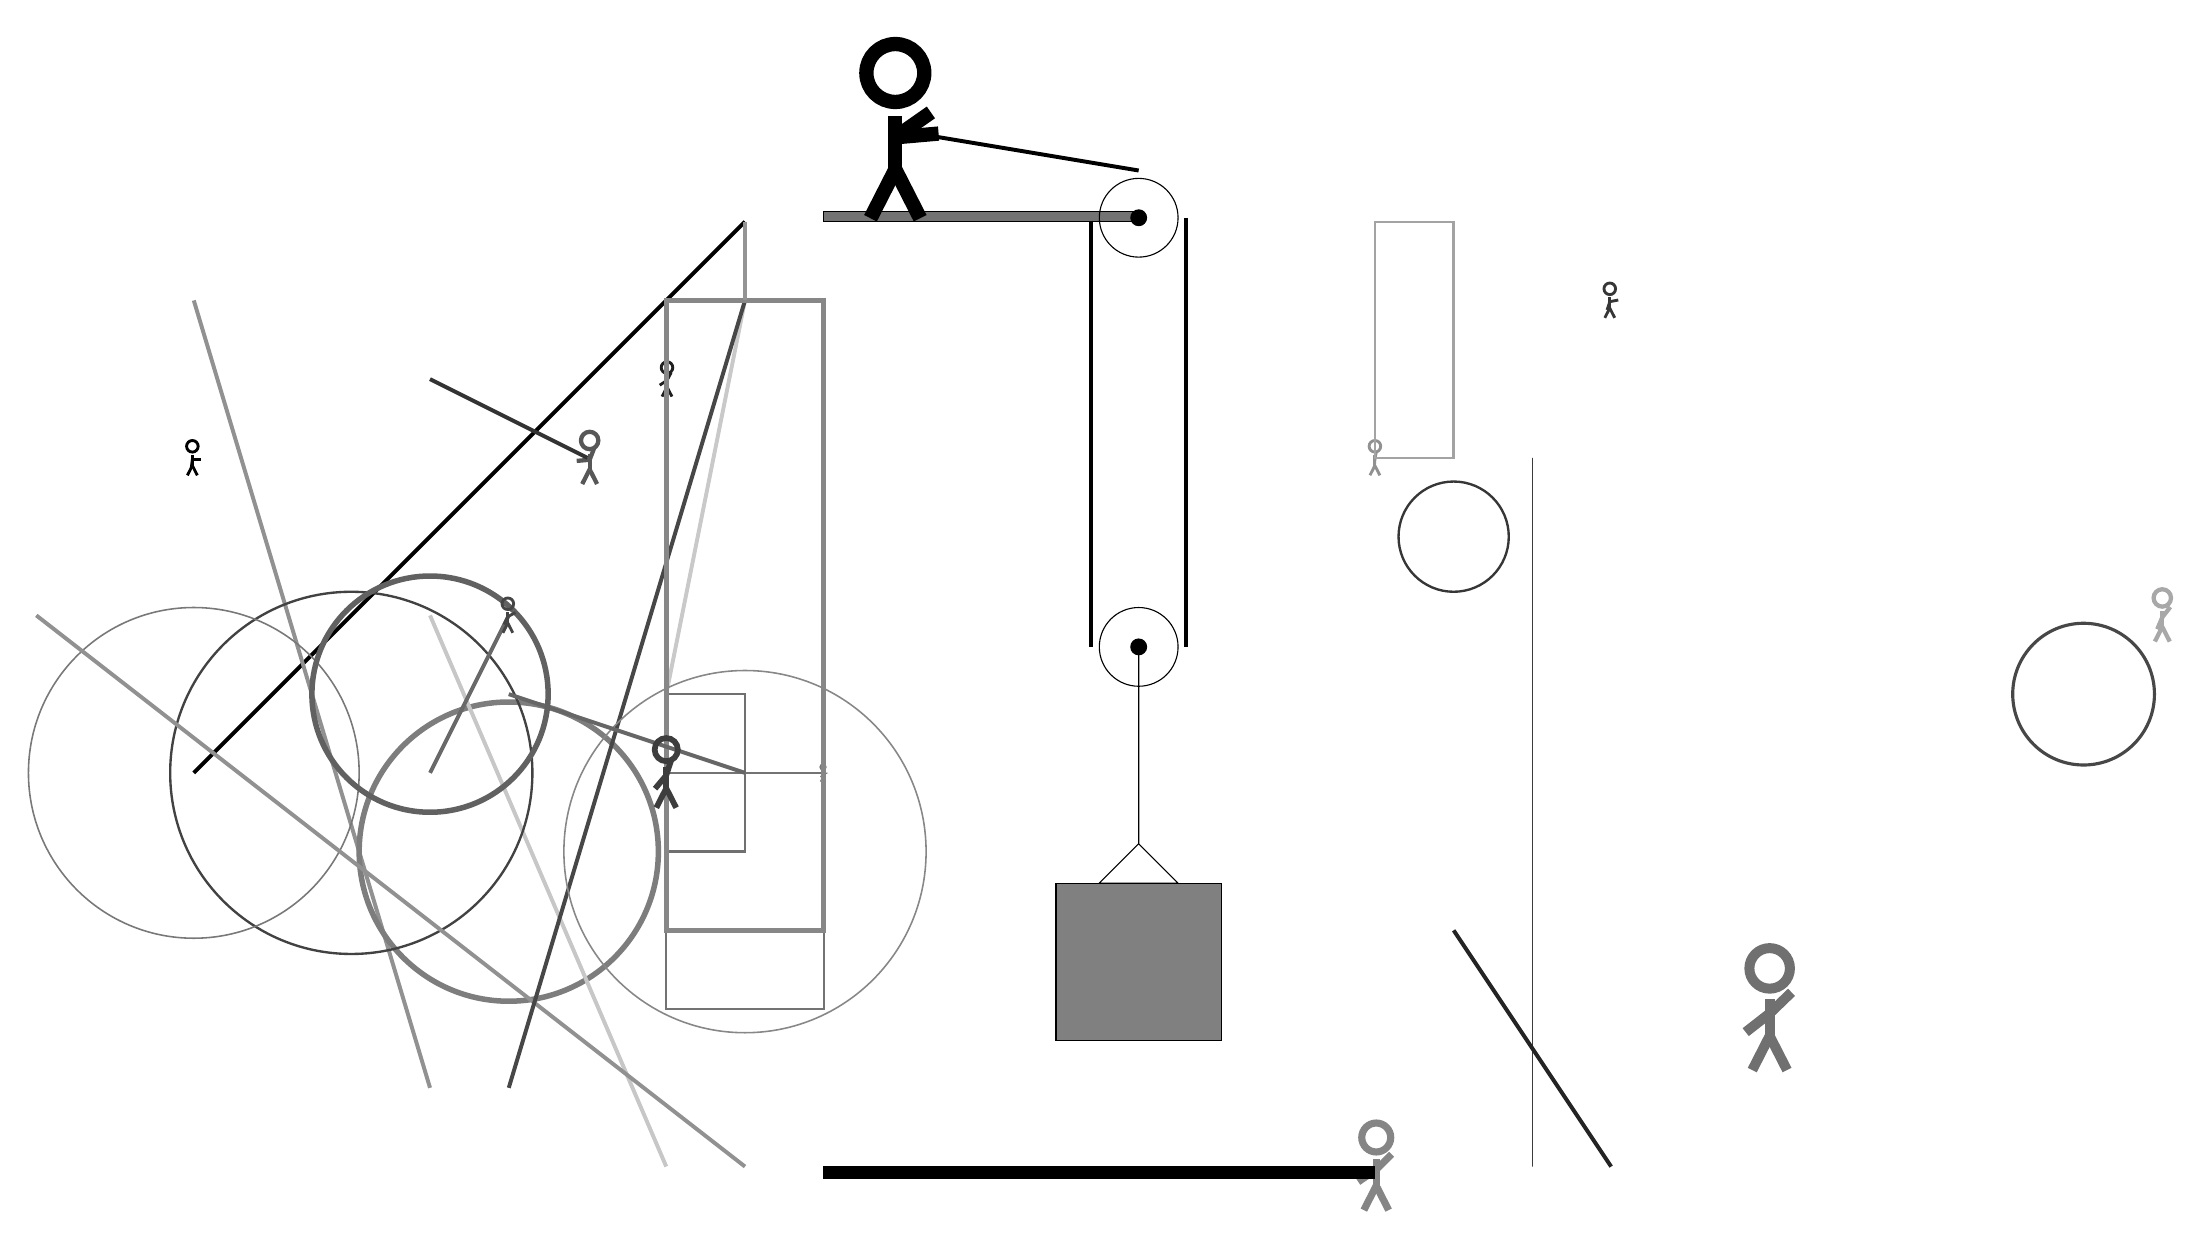
\begin{tikzpicture}
			%%%%% START %%%%%
			
			\draw[fill=black!55] (-2, 9) rectangle (2, 9.125);
			
			\draw (2, 3.6) circle (0.5);
			\draw[fill=black] (2, 3.6) circle (0.1);
			
			\draw (2, 9.05) circle (0.5);
			\draw[fill=black] (2, 9.05) circle (0.1);
			
			\draw (2, 3.6) -- (2, 1.1) -- (1.5, 0.6) -- (2.5, 0.6) -- (2, 1.1);
			\draw[fill=black!50] (0.95, 0.6) rectangle (3.05, -1.4);
			
			\draw[line width=0.5mm] (1.4, 9) -- (1.4, 3.6);
			\centerarc[line width=0.5mm](2, 3.6)(180:360:0.6);
			\draw[line width=0.5mm](2.6, 3.6) -- (2.6, 9.05);
			\centerarc[line width=0.5mm](2, 9.05)(0:90:0.6);
			\draw[line width=0.5mm](2, 9.65) -- (-1, 10.15);
			
			\draw[line width=0.3mm, color=black!56] (-4, 3) rectangle (-3, 1);
			
			\draw[line width=0.5mm, color=black!100](-3, 9) -- (-10, 2);
			\node[line width=0.2mm, color=black!79] at (8, 8) {\Strichmaxerl[2][72][11]};
			\draw[line width=0.5mm, color=black!43](-7, -2) -- (-10, 8);
			\draw [line width=0.7mm, color=black!51](-6, 1) circle (1.9);
			\draw[line width=0.2mm, color=black!77] (7, 6) rectangle (7, -3);
			
			\draw[line width=0.5mm, color=black!22](-7, 4) -- (-4, -3);
			\draw [line width=0.3mm, color=black!74](-8, 2) circle (2.3);
			\draw [line width=0.2mm, color=black!53](-10, 2) circle (2.1);
			\draw[line width=0.5mm, color=black!21](-4, 3) -- (-3, 8);
			
			\node[line width=0.2mm, color=black!53] at (-2, 2) {\Strichmaxerl[1][57][4]};
			\draw[line width=0.5mm, color=black!43](-3, -3) -- (-12, 4);
			\node[line width=0.7mm, color=black!66] at (-5, 6) {\Strichmaxerl[3][5][69]};
			
			\node[line width=0.2mm, color=black!56] at (10, -1) {\Strichmaxerl[7][38][44]};
			\draw[line width=0.5mm, color=black!59](-7, 2) -- (-6, 4);
			\draw[line width=0.3mm, color=black!55] (-4, 2) rectangle (-2, -1);
			\draw[line width=0.5mm, color=black!72](-6, -2) -- (-3, 8);
			\node[line width=0.3mm, color=black!43] at (5, 6) {\Strichmaxerl[2][86][79]};
			\node[line width=0.5mm, color=black!48] at (5, -3) {\Strichmaxerl[5][34][45]};
			\draw [line width=0.2mm, color=black!47](-3, 1) circle (2.3);
			\draw[line width=0.3mm, color=black!36] (5, 9) rectangle (6, 6);
			\draw [line width=0.4mm, color=black!72](14, 3) circle (0.9);
			\node[line width=0.5mm, color=black!88] at (-4, 7) {\Strichmaxerl[2][33][62]};
			\draw[line width=0.6mm, color=black!47] (-2, 0) rectangle (-4, 8);
			\draw [line width=0.3mm, color=black!79](6, 5) circle (0.7);
			
			\draw[line width=0.5mm, color=black!86](8, -3) -- (6, 0);
			
			\node[line width=0.5mm, color=black!34] at (15, 4) {\Strichmaxerl[3][67][52]};
			\draw[line width=0.5mm, color=black!60](-6, 3) -- (-3, 2);
			\draw[line width=0.5mm, color=black!80](-7, 7) -- (-5, 6);
			\node[line width=0.5mm, color=black!76] at (-4, 2) {\Strichmaxerl[4][50][72]};
			\draw[line width=0.5mm, color=black!42](-3, 9) -- (-3, 8);
			
			\draw [line width=0.7mm, color=black!62](-7, 3) circle (1.5);
			\node[line width=0.3mm, color=black!100] at (-10, 6) {\Strichmaxerl[2][83][0]};
			\node[line width=0.2mm, color=black!73] at (-6, 4) {\Strichmaxerl[2][64][28]};
			
			\node at (-1, 10.15) {\Strichmaxerl[10][-175][35]};
			
			\draw[fill=black] (-2, -3) rectangle (5, -3.15);
			
			%%%%% END %%%%%
		\end{tikzpicture}
	\end{figure}	
\end{document}